\section{Durchführung}
Für den experimentellen Aufbau wird im wesentlichen eine Kupfer-Röntgenröhre, ein LiF-Kristall und ein Geiger-Müller-Zählrohr benötigt. In dem Röntgengerät aus Abbildung \ref{fig:aufbau}
sind die Teile bereits verbaut und können mit einem Rechner oder manuell bedient werden.
\begin{figure}
    \centering
    \caption{Versuchsaufbau zur Messung von Röngenspektren \cite{V602}}
    \label{fig:aufbau}
    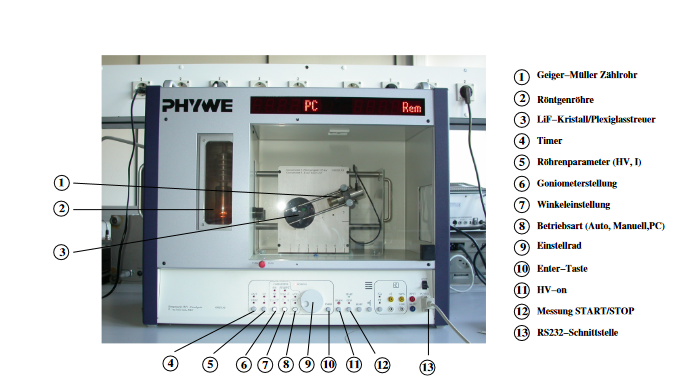
\includegraphics[width = 0.6 \textwidth]{pics/gerät.png}
\end{figure}
An der Röntgenröhre wird eine Beschleunigungsspannung von $U_\text{B}=\SI{35}{\kilo \volt}$ und ein Emissionsstrom von $I=\SI{1}{\milli\ampere}$ eingestellt.
Vor der Messung wird noch einmal überprüft, ob die $\SI{1}{\milli\metre}$ Blende und der LiF-Kristall in den Halterungen stecken und korrekt ausgerichtet sind.
Für die Absorptionsmessungen werden Blenden mit verschiedenen Absorbern vor das Geiger-Müller Zählrohr angebracht.
\\
Um die Bragg Bedingung zu überprüfen, wird der LiF-Kristall auf einen festen Kristallwinkel von $\theta=\ang{14;;}$ gestellt. Das Geiger-Müller Zählrohr misst in einem Winkelbereich von 
$\alpha_\text{GM}=\ang{26;;} $ bis $\alpha_\text{GM}=\ang{30;;} $ mit einem Winkelzuwachs von $\symup{\Delta} \alpha =\ang{0.2;;}$. Als Integrationszeit pro Winkel wird 
$\symup{\Delta}t=\SI{5}{\second}$ genutzt.
\\
Im Programm wird der 2:1 Koppelmodus angewählt.
Um das Emissionsspektrum der Cu-Röntgenröhre zu bekommen, wird das Röntgenspektrum im Winkelbereich $\ang{8;;} \leq \theta \leq \ang{25;;}$ in $\ang{0.1;;}$
-Schritten unter einer Integrationszeit von $\symup{\Delta}t=\SI{10}{\second}$ gemessen. Dadurch ist auch keine zusätzliche Messung des Detailspektrums der $K_\alpha$
und $K_\beta$ Linien von Kupfer nötig.
\\
In der letzten Messreihe werden verschiedene Absorber zwischen den LiF-Kristall und das Geiger-Müller Zählrohr eingesetzt. Dabei werden Absorber aus Zink, Gallium, Brom, Rubidium und Stronzium verwendet.
Die Absorptionsspektren werden bei einer Integrationszeit von $t=\SI{20}{\second}$ gemessen. Für die verschiedenen Materialien werden individuelle Winkelbereiche genutzt.